% 01-introduction.tex — truth: 本文件（2026-11-15 深度改造：主张收缩为 taxonomy 演化下物理-语义解耦的成本-收益边界与透明评估协议；犬类负结果前置为边界条件；贡献列表同步收缩）
% 纪律: Para1-6 六段式逐块搬运; Hero figure fig1 落 §1 尾（figure-specs.md 规格）; 数字禁改写。
% Abstract 已在 main.tex 前置区，本节从 Introduction 正文开始。label 沿用桩定义 sec:intro。
\section{Introduction}\label{sec:intro}

Deployed behavior-recognition pipelines rarely face a fixed definition of what they recognize. Working-dog programs redefine behavior categories as training standards evolve; welfare protocols split or merge classes as regulations change; veterinary research adopts finer ethograms as instruments improve. Each such revision re-opens the annotation and retraining pipeline behind the classifier. The economics are unforgiving: training a working dog costs tens of thousands of dollars per animal, and more than half of candidates fail to graduate~\citep{grimm2026science}, so the measurement layer around these programs is both expensive and subject to recurring re-specification.

This paper studies a structural response to that recurring cost: factorize the pipeline so that the part that must track the taxonomy is small. We examine the physics--semantics decoupling pattern, PSD, for skeleton-based behavior recognition under evolving evaluation criteria. A physics layer $\Phi$ learns \emph{how skeletons move} without behavior labels: self-supervised pretraining adapted to quadruped topology plus unsupervised motion-word segmentation that cuts streams into behavior proposals. A semantic layer $\Omega$ learns \emph{what behaviors are called} from a small seed budget: rule-engine coarse labels seed class anchors, prototype clustering assigns pseudo-labels under confidence filtering, and iterated expansion operates within an annotation budget of 100--200 clips; a warm-start protocol initializes this stage from prior semantic-layer weights, making budgets as small as 20 clips usable on the synthetic-offset tier (the canine-tier outcome at a comparable budget is reported in Section~\ref{sec:experiments}). Because the layers interact only through embeddings and proposals, a taxonomy transition $\mathcal{Y}\to\mathcal{Y}'$ retrains $\Omega$ while $\Phi$ remains frozen.

The question this paper answers is deliberately narrower than ``does decoupling work?''. Any design that freezes a backbone and retrains a head inherits the same computational shortcut at a taxonomy change, so the wall-clock ratio alone does not justify the mechanism; and a pre-registered real-domain replication shows the shortcut can invert at small scale, where there is no retraining cost left to save (Section~\ref{sec:experiments}, E6-real). We therefore treat decoupling as a cost--benefit hypothesis with explicit boundary conditions: it pays where a frozen physics layer remains reusable and semantics are cheap to rebuild, and it fails where pseudo-label quality collapses. The contribution is a measured boundary (where the cost advantage holds, where accuracy holds, and where the pipeline breaks), established under a pre-registered, tier-separated protocol whose decision rules, tolerances, and negative results are reported in full.

\paragraph{Why animal skeletons, and where the boundary lies.}
Animal behavior recognition motivates the problem: labeled behavior data is scarce, skeletons are the practical signal, and evaluation criteria in working-dog and welfare settings evolve with operational practice (Section~\ref{ssec:rw-animal}). On the only public canine behavior tier we could assemble, the end-to-end pipeline stays below chance at a 13\% annotation budget (\textbf{9.8\% $\pm$ 7.5 against an 11.1\% chance level}, with a generic-SSL control reaching \textbf{15.2\% $\pm$ 5.1}), and a pre-registered diagnosis attributes the failure to label misalignment in the sole public source of canine behavior video with action labels, not to skeleton quality (Section~\ref{sec:experiments}, E7; Section~\ref{sec:conclusion}, L9). We report this as a boundary condition, have pre-registered the target-domain working-dog pilot for a later study, and scope every positive claim to the tiers where it was actually measured rather than claiming a general solution to animal behavior recognition.

Our contributions are threefold:
\begin{enumerate}
\item \textbf{A cost--benefit boundary for physics--semantics decoupling under taxonomy evolution.} On the synthetic tier, a taxonomy transition is absorbed at $\geq 3\times$ lower wall-clock retraining cost than full-pipeline retraining at matched accuracy (conservative bound backed by a measured $6.07\times$; same-seed paired ratios never below $3.99\times$). This bound is a synthetic-tier measurement: real-domain replications return FAIL at MLP scale (no cost to save) and PARTIAL at backbone scale (cost line cleared, accuracy band not exactly matched), so the claim is scoped, not universal.

A pre-registered merge/rename analysis sharpens the boundary. For transitions expressible as label remaps or logit aggregation, zero-retraining upper bounds apply. On the one real merge transition we measure, a matched-solver control bounds the decoupled rebuild from above (82.6\% vs.\ 75.3\%), and the zero-retraining remap bound measured on the same episode reads 68.0\%, below the rebuild; the rebuild is therefore not dominated by the zero-cost path on this episode.

A synthetic split/addition episode probes the residual value of decoupling where new supervision is unavoidable: the zero-retraining remap cannot name the new classes (0\%), and the decoupled rebuild recovers 45.7\% overall with 10 new labels per class, at $3.0\times$ lower median wall-clock and $5\times$ fewer new labels than full retraining (97.1\%; a frozen head with the full new-label budget: 68.0\%). A labeled-budget ladder on the same transition type ($k\in\{10,25,50,100\}$ fresh labels per new class) raises the decoupled arm from 45.3\% to 72.4\% (three seeds 42--44 per rung) but saturates at the frozen-feature ceiling (frozen-head arm: 71.7\%) and never approaches the coupled arm (95.9\%). The smallest margin, 23.45\,pp at $k{=}100$, sits far outside the $\pm2.3$\,pp parity band, so the residual-value hypothesis fails across the entire tested ladder; decoupling's measured value in this regime is label and wall-clock savings, and closing the gap appears to require adapting the frozen encoder (seeds 42--44; Section~\ref{sec:experiments}).

The cost of freezing itself is likewise measured. A frozen-encoder control on the three real E9-series tiers (NTU120, UCF101, PanAf500) shows naive freezing retains only \textbf{88.9\%/66.6\%/85.8\%} of full-budget accuracy under the interim supervised encoder, and a protocol-return amendment executing the pre-registered label-free physics layer on NTU120, UCF101, and PanAf500 reads \textbf{75.0\%/51.1\%/82.5\%} (all \textbf{FAILS}; Section~\ref{ssec:boundary}).
%% [E3-INTERFACE·已消费 2026-11-16] 贡献1 的假设从句已按 E3 实测替换为实证句：
%%   remap 新类 0% / decoupled(k=10) 45.7% @100 新标注（三种子 0.4448/0.4345/0.4931 均值 0.45747，两位小数 45.75%）/ frozen head 68.0% / coupled 97.1%；
%%   墙钟中位 50.6s vs 153.0s = 3.0×；新标注 100 vs 500 = 5×。seeds 42/43/44。
%% 数值源: runs/p1_sprint/split_addition_episode/summary.json（reports/p1_sprint_evidence/ 有逐字节一致副本）。
%% [E3b-INTERFACE·已消费 2026-11-16] 贡献1 剩余价值句按 k 阶梯（E3b）实测降级：
%%   decoupled 45.3/59.1/65.1/72.4%（k=10/25/50/100；全部档位三种子 42/43/44，std ddof=0；k=100 ±0.0），coupled 95.9%（±0.5，k 无关参照），
%%   frozen-head 71.7%；最小边际 23.45pp@k=100，全梯度落在 ±2.3pp 平价带外 → k*=None，
%%   verdict=no_parity_within_tested_range → "residual-value hypothesis not supported at any tested budget"。
%% 数值源: runs/p1_sprint/k_ladder/summary.json（reports/p1_sprint_evidence/ 有副本），严禁编造。
%% 三处联动已同步（2026-11-16 统稿）: main.tex 摘要句（同 episode 界 68.0%@10% 标注头预算 + E3/E3b 降级式剩余价值）与
%% 06-conclusion-limitations.tex（结论段 + L12）均已改为同口径；60→10 的 76.8% 仅保留为另一 episode 的合法数字。
%% [FROZEN-REAL·已消费 2026-11-16] 贡献1 尾句新增冻结代价实测: 三真实 tier frozen-encoder 对照 88.9/66.6/85.8%（PARTIAL/FAILS/PARTIAL）。
%% 数值源: runs/p1_sprint/{ntu120,ucf101,panaf500}/summary.json（与 2026-09-07 已报告 E9 值逐位一致）;
%% 正文载体: ssec:boundary 冻结对照 bullet + tab:attribution-controls 真实 tier 块; 协议全文 supplementary app:frozenreal。
\item \textbf{A transparent, pre-registered evaluation protocol for tier-separated claims.} Three tiers (synthetic, public-real, real-K9) plus public benchmarks are never pooled; every comparison carries its caliber (label space, budget definition, device, seed dispersion); cost is reported as a pair (annotation units, wall-clock) at matched accuracy; and decision rules (including the conservative $\geq 3\times$ bound, the FULL/PARTIAL/FAIL verdicts, and Holm-corrected families) are frozen before runs. Negative results are first-class findings: the canine-tier collapse below chance, the null rescue levers, and the retention collapse on weak-reference domains (UCF101 66.6\% interim encoder; 51.1\% label-free) are reported under the same rules that certify the positive results.
\item \textbf{An honest empirical map of where the mechanism pays.} Positive evidence: the warm-started semantic layer reaches 82.0\% top-1 on 22 classes from 20 labeled clips on the synthetic-offset tier (vs.\ 96.6\% full-budget; a marginal budget atop a fully labeled source domain), and the end-to-end pipeline retains 90.7\% of full-budget linear-probe accuracy at 10\% of the labels on the human benchmark (75.0\% on NTU120 under the pre-registered label-free physics layer, vs.\ 88.9\% under a disclosed interim supervised encoder; 85.8\% on PanAf500 at thirty seeds (interim encoder; 82.5\% under the pre-registered label-free physics layer), ten-seed readout released alongside); separately, a linear head on frozen features alone retains 88.7\% on NTU60. Under the identical budget protocol the 10\% semantic arm also edges re-implemented published-method baselines, AimCLR linear evaluation (67.5\% vs.\ 66.7\%) and end-to-end supervised ST-GCN (64.8\%), while full-budget supervision dominates (83.5\%; Table~\ref{tab:h2h}). Boundary evidence: on the canine public-real tier the same corrected protocol stays below chance (9.8\% vs.\ 11.1\%) with a generic-SSL control ahead (15.2\%), and the pre-registered working-dog tier remains untested. Together these delineate the regime in which decoupled, low-budget semantic expansion is worth deploying, and the regime in which it is not (Sections~\ref{sec:experiments}--\ref{sec:ablation}).
\end{enumerate}

Figure~\ref{fig:framework} illustrates the framework. Section~\ref{sec:related} reviews related work. Section~\ref{sec:method} details the method. Sections~\ref{sec:experiments}--\ref{sec:ablation} report experiments and ablations, and Section~\ref{sec:conclusion} concludes with limitations.

\begin{figure}[pos=htbp]
  \centering
  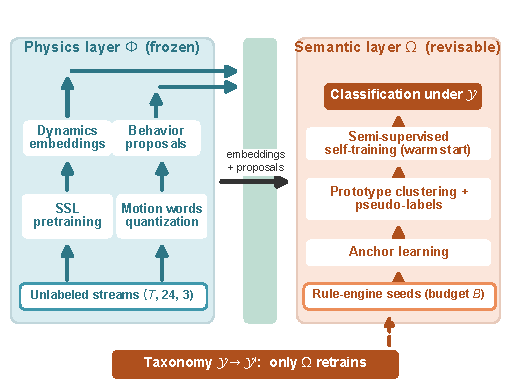
\includegraphics[width=0.76\linewidth]{fig1_framework_overview.pdf}
  \caption{The PSD framework. A frozen physics layer $\Phi$ (left) turns unlabeled skeleton streams into dynamics embeddings and behavior proposals via self-supervised pretraining and motion-word quantization. A revisable semantic layer $\Omega$ (right) expands rule-engine seeds into taxonomy coverage through anchor-guided clustering with iterated confidence-filtered pseudo-labeling, consolidated by self-training and warm-started small-budget initialization. The layers communicate only through embeddings and proposals, so a taxonomy transition $\mathcal{Y}\to\mathcal{Y}'$ retrains $\Omega$ alone.}\label{fig:framework}
\end{figure}
